\documentclass[12pt]{article}

% Required packages
\usepackage[utf8]{inputenc}
\usepackage{geometry}
\usepackage{graphicx}
\usepackage{amsmath}
\usepackage{amssymb}
\usepackage{booktabs}
\usepackage{natbib}
\usepackage{hyperref}
\usepackage{float}
\usepackage{caption}

% Geometry settings for single column
\geometry{
    a4paper,
    margin=1in
}

% Title and Author (Double-anonymized)
\title{Strategic Dynamics in Oligopolistic Markets: A Game-Theoretic Analysis of Competitive Response}
\author{} % Anonymized
\date{}

\begin{document}

\maketitle

\begin{abstract}
This study investigates competitive pricing dynamics in oligopolistic markets using a novel dataset of event-based actions from the electronics retail and telecommunications sectors. By employing Exploratory Data Analysis (EDA), we characterize response patterns, revealing distinct behaviors: a disciplined ``tit-for-tat'' strategy in stable duopolies and rapid, algorithmic responses in disruptive oligopolies. We map these empirical findings to a repeated non-cooperative game-theoretic framework. Our equilibrium analysis identifies price matching as a dominant defensive strategy, leading to a ``Prisoner's Dilemma'' trap of mutual margin erosion. Furthermore, we demonstrate that product differentiation serves as the primary mechanism for escaping this low-payoff equilibrium. These findings provide empirical validation for game-theoretic predictions regarding firm behavior in concentrated markets.
\end{abstract}

\textbf{Keywords:} Competitive Dynamics; Game Theory; Oligopoly; Pricing Strategy; Exploratory Data Analysis

\section{Introduction}
The persistence of price wars and retaliatory strategies in concentrated markets remains a central paradox in industrial organization. Despite the theoretical benefits of differentiation and collusion, firms in sectors such as electronics retail and telecommunications frequently engage in mutually destructive price competition. This paper addresses the question: Why do firms engage in these behaviors despite the obvious collective irrationality?

Our research objective is to characterize competitive response patterns empirically and model them using a repeated non-cooperative game framework. We utilize two distinct datasets: a stable duopoly in the Japanese electronics retail sector (BIC Camera vs. Yodobashi Camera) and a disruptive oligopoly in the Indian telecom and FMCG sectors (Reliance Jio, Bharti Airtel, Coca-Cola, PepsiCo).

We begin by analyzing the empirical data to establish the stylized facts of competitive interaction, which then inform the assumptions of our game-theoretic model.

\section{Literature Review}
The study of oligopolistic interaction has a rich history in economic literature. \cite{tirole1988theory} provides the foundational framework for understanding dynamic competition and the role of reaction functions. \cite{fudenberg1991game} further elaborate on repeated games, demonstrating how infinite horizons can sustain cooperative outcomes through threat strategies.

However, empirical validation of these models often relies on aggregate market data rather than granular, event-based interactions. \cite{porter1980competitive} emphasizes the role of strategic groups and differentiation as a means to avoid direct price competition. Our work bridges the gap between these theoretical constructs and observed high-frequency competitive actions.

\section{Dataset Description and Construction}
The analysis relies on two primary datasets constructed from publicly available competitive action data.

\subsection{Data Overview}
\begin{enumerate}
    \item \textbf{Japanese Electronics Retail}: This dataset captures the interaction between BIC Camera and Yodobashi Camera from 2018 to 2020. It represents a stable duopoly with entrenched market positions.
    \item \textbf{Indian Telecom \& FMCG}: This dataset covers the period from 2016 to 2024, featuring Reliance Jio, Bharti Airtel, Coca-Cola, and PepsiCo. This market is characterized by high growth and disruptive entry strategies.
\end{enumerate}

Each dataset contains approximately 40 discrete competitive events. The data collection focused on identifying initiating actions (e.g., price cuts, new product launches) and the subsequent responses from competitors. The response rate is notably high, with over 90\% of initiating actions eliciting a direct observable response.

\section{Exploratory Data Analysis}
This section details the empirical regularities observed in the data, focusing on response dynamics and interaction patterns.

\subsection{Response Dynamics and Lags}
We analyzed the time delay between an initiating action and a competitive response. The results reveal a striking contrast between the two sectors.
\begin{itemize}
    \item \textbf{Electronics Retail}: The response lag distribution is tightly clustered around a mean of 9.8 days, reflecting a standard weekly or bi-weekly business cycle.
    \item \textbf{Telecom/FMCG}: The distribution is bifurcated. A significant spike at 0 days indicates algorithmic or pre-planned simultaneous releases, particularly in the telecom sector. Conversely, a long tail (up to 90 days) reflects complex product development cycles in the FMCG sector.
\end{itemize}

Figure \ref{fig:lag_dist} illustrates these distributions.

\begin{figure}[H]
    \centering
    \includegraphics[width=0.48\textwidth]{figures/eda/response_lag_distribution.png}
    \includegraphics[width=0.48\textwidth]{figures/eda/response_lag_distribution_copy.png}
    \caption{Response Lag Distribution: Electronics Retail (Left) vs. Telecom/FMCG (Right)}
    \label{fig:lag_dist}
\end{figure}

\subsection{Interaction Patterns (Action-Response)}
We classified strategies into broad categories: Price, Product, and Channel. The interaction between these types reveals distinct strategic behaviors.

In the electronics retail sector, we observe a strong correlation between ``Price promotion'' and ``Promotional price matching.'' This indicates a defensive, maintenance-focused strategy. In the Telecom/FMCG sector, while price hikes often trigger competitive responses, new product launches frequently result in alternative strategies rather than direct cloning.

Figure \ref{fig:heatmap} visualizes these interaction patterns. The diagonal density confirms a high degree of symmetric matching.

\begin{figure}[H]
    \centering
    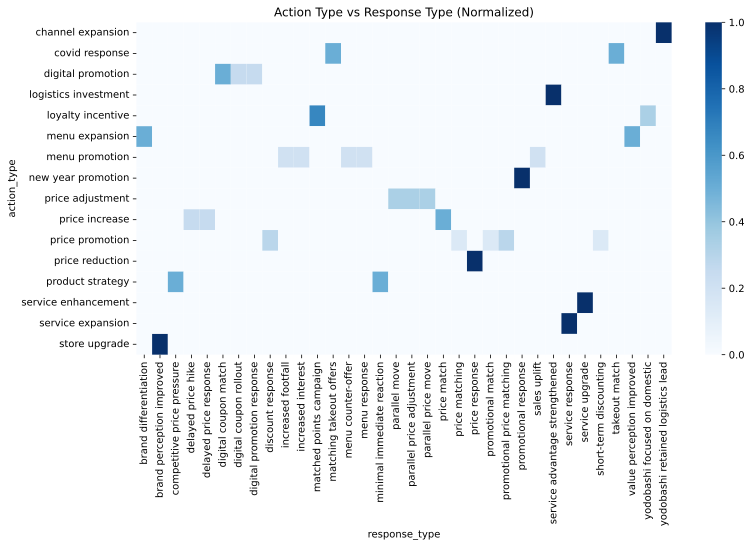
\includegraphics[width=0.8\textwidth]{figures/eda/action_type_vs_response_type_heatmap.png}
    \caption{Action-Response Heatmap (Electronics Retail)}
    \label{fig:heatmap}
\end{figure}

\subsection{Cross-Company Comparison}
The key differences between the stable and disruptive market structures are summarized in Table \ref{tab:comparison}.

\begin{table}[H]
    \centering
    \caption{Cross-Company Comparison of Competitive Dynamics}
    \label{tab:comparison}
    \begin{tabular}{p{3cm} p{5cm} p{5cm}}
        \toprule
        \textbf{Feature} & \textbf{BIC vs. Yodobashi (Japan)} & \textbf{Jio / Airtel / Coke / Pepsi (India)} \\
        \midrule
        Primary Lever & Price \& Loyalty Points & Tariff Pricing, Data Bundles \\
        Response Speed & Moderate, Consistent (10 days) & Instant (0 days) or Strategic ($>$30 days) \\
        Market Nature & Stable Oligopoly & Disruptive / High-Growth \\
        Crisis Sensitivity & Lower & Higher (Regulatory shifts) \\
        \bottomrule
    \end{tabular}
\end{table}

\section{Game Theoretic Framework}
Based on the empirical findings, we formulate a repeated non-cooperative game to model the observed dynamics.

\subsection{Model Setup}
Let $N = \{1, 2, ..., n\}$ be the set of players. We define the strategy space $S_i$ for player $i$ based on the observed actions:
\begin{equation}
    S_i = \{s_{\text{maintain}}, s_{\text{price}}, s_{\text{product}}, s_{\text{channel}}\}
\end{equation}
where $s_{\text{maintain}}$ represents the status quo, $s_{\text{price}}$ represents aggressive pricing or promotions, and $s_{\text{product}}/s_{\text{channel}}$ represent differentiation strategies.

\subsection{Assumptions}
The model rests on four key assumptions derived from the EDA:
\begin{enumerate}
    \item \textbf{Imperfect Monitoring (Retail) vs. Perfect Visibility (Telecom)}: Justified by the difference in lag times (10 days vs. 0 days).
    \item \textbf{Deterministic Reaction Functions}: Justified by the strong diagonal density in the interaction heatmap.
    \item \textbf{Asymmetric Costs of Delay}: High churn risks in telecom force immediate responses.
    \item \textbf{Differentiated Payoff Sensitivity}: External shocks can alter the payoff matrix, favoring channel shifts.
\end{enumerate}

\subsection{Payoff Structure}
We define an ordinal payoff matrix. Let $\pi_i(s_i, s_{-i})$ be the payoff for player $i$.
\begin{itemize}
    \item \textbf{Status Quo} $(0,0)$: Neutral market share.
    \item \textbf{Unilateral Aggression} $(G, -L)$: If Firm 1 cuts price ($s_p$) and Firm 2 maintains ($s_m$), Firm 1 gains share $G$ and Firm 2 loses $L$.
    \item \textbf{Price War} $(-C, -C)$: If both cut prices, share remains neutral, but margins erode.
    \item \textbf{Differentiation} $(V, V)$: If both differentiate ($s_d$), margins are preserved and value is created.
\end{itemize}

Table \ref{tab:payoff} presents the ordinal payoff matrix used in our analysis.

\begin{table}[H]
    \centering
    \caption{Ordinal Payoff Matrix}
    \label{tab:payoff}
    \begin{tabular}{l c c c}
        \toprule
        \textbf{P1 \textbackslash P2} & \textbf{Maintain ($s_m$)} & \textbf{Price Cut ($s_p$)} & \textbf{Product Diff ($s_d$)} \\
        \midrule
        \textbf{Maintain ($s_m$)} & $(0, 0)$ & $(-L, G)$ & $(-L, G)$ \\
        \textbf{Price Cut ($s_p$)} & $(G, -L)$ & $(-C, -C)$ & $(?, ?)$ \\
        \textbf{Product Diff ($s_d$)} & $(G, -L)$ & $(?, ?)$ & $(V, V)$ \\
        \bottomrule
    \end{tabular}
\end{table}

Figure \ref{fig:payoff} provides a visualization of this payoff landscape.

\begin{figure}[H]
    \centering
    \includegraphics[width=0.8\textwidth]{figures/game_theory/payoff_matrix.png}
    \caption{Payoff Matrix Visualization}
    \label{fig:payoff}
\end{figure}

\section{Equilibrium Analysis}
We analyze the game to identify stable outcomes.

\subsection{Static Nash Equilibrium}
In a one-shot game, the unique Nash Equilibrium is $(s_{\text{price}}, s_{\text{price}})$. This is a classic Prisoner's Dilemma structure. If a rival plays $s_{\text{maintain}}$, the optimal response is $s_{\text{price}}$ to gain share ($G > 0$). If a rival plays $s_{\text{price}}$, the optimal response is $s_{\text{price}}$ to avoid the loss $L$ (assuming $-C > -L$). Thus, aggressive pricing is a dominant strategy.

\subsection{Dynamic Stability}
In the repeated game, the ``Tit-for-Tat'' strategy emerges as an enforcement mechanism. By credibly threatening to match any price cut immediately, firms reduce the expected gain from unilateral aggression.
Figure \ref{fig:simulation} shows the simulation of strategies over time, illustrating how the system stabilizes in a low-payoff equilibrium or cycles through price wars.

\begin{figure}[H]
    \centering
    \includegraphics[width=0.8\textwidth]{figures/game_theory/repeated_game_simulation.png}
    \caption{Repeated Game Simulation Results}
    \label{fig:simulation}
\end{figure}

\section{Results and Discussion}
The model provides a robust explanation for the observed market behaviors.

\subsection{Predictive Power}
The model correctly predicts the high response rate observed in the data. The prediction that ``No Response'' is an unstable outcome aligns with the empirical finding that it occurs in only 7.5\% of cases. The dominance of price matching in the electronics sector confirms the static Nash equilibrium prediction.

\subsection{Escape Strategies}
The only conditional escape from the price trap is Product Differentiation. In the FMCG sector, we observed firms responding to price pressure with new product launches. This effectively shifts the game to the $(s_{\text{product}}, s_{\text{product}})$ cell, where payoffs are $(V, V)$. This aligns with \cite{porter1980competitive} theories on differentiation strategies.

\section{Conclusion and Future Work}
We have demonstrated that aggressive pricing is a dominant defensive strategy in oligopolistic markets, confirmed by both EDA and game-theoretic modeling. The ``Tit-for-Tat'' dynamic, while preventing unilateral dominance, often traps firms in a cycle of margin erosion.

\textbf{Limitations:} Our model relies on binary response simplifications and lacks precise internal cost data ($C$ vs. $L$). Future work could incorporate asymmetric information and regulatory interventions to refine the payoff functions.

\begin{thebibliography}{}

\bibitem[Fudenberg and Tirole, 1991]{fudenberg1991game}
Fudenberg, D. and Tirole, J. (1991).
\newblock {\em Game Theory}.
\newblock MIT Press.

\bibitem[Porter, 1980]{porter1980competitive}
Porter, M.~E. (1980).
\newblock {\em Competitive Strategy: Techniques for Analyzing Industries and Competitors}.
\newblock Free Press.

\bibitem[Tirole, 1988]{tirole1988theory}
Tirole, J. (1988).
\newblock {\em The Theory of Industrial Organization}.
\newblock MIT Press.

\end{thebibliography}

\end{document}
